\documentclass[10pt,twocolumn]{article}
\usepackage{ctex}
\usepackage{graphicx}
\usepackage{algorithm}
\usepackage{algorithmic}
\usepackage{amssymb}
\usepackage{amsmath}
\usepackage{hyperref}
\usepackage{mathrsfs}

\begin{document}
\title{\textbf{高斯过程回归及其应用}}
%\subtitle{概率论与随机过程(2)  第二次大作业}
\author{无47\hspace{2em}刘前\thanks{E-mail: liuqian14@mails.tsinghua.edu.cn,清华大学电子工程系。}\hspace{2em}2014011216\hspace{2em}}
\date{}

\maketitle

\noindent{\kaishu\small{{\heiti 摘要:}高斯过程回归是一种重要的回归分析方法。本文重点关注对高斯过程回归的应用,解决了两个问题。第一个问题中实现了对一维数据的建模,先比较了不同基本核函数的效果,然后通过核函数的加法、乘法复合,对训练数据建模,以测试数据MSE最低的原则得到了相对最优的核函数模型。第二个问题中,设计了使用高斯过程回归解决高维问题的方法,比较了Laplace近似、变分贝叶斯及LOO交叉验证共计三种贝叶斯推断近似方法的效果,每种近似方法下都比较了不同的均值函数、核函数和似然函数,最终在测试数据上比较MSE得到了最优选择。
}}

\section{基本介绍}

\subsection{回归分析}
回归分析(Regression Analysis)是一种应用广泛的统计分析方法,主要研究两种或两种以上变量之间相互依赖的定量关系,目前是统计学、信号处理及机器学习等众多领域的重要研究方法之一。

回归分析的主要目的是确定自变量$\mathbf{x}\in\mathbf{S}\subset{\mathbb{R}^{d}}$与因变量$y\in\mathbb{R}$之间的函数关系$y=f(\mathbf{x})+e$。
其中$f(x)$称为回归函数(或拟合函数),$e$为误差随机变量。回归分析的关键和难点在于确定回归函数$f(x)$的具体形式。一般来说,回归函数的选取准则可以归结为:给定一组训练数据$\mathscr{D} = \{(x_{i},y_{i})\vert i = 1,2,\cdots,n\}$,在某些准则下根据训练数据确定最好的回归函数$f(\mathbf{x})$及相应参数。回归分析的步骤为:

{\romannumeral1}.{\kaishu 确定合适的回归函数形式;}

{\romannumeral2}.{\kaishu 根据训练数据求出具体的回归函数(确定函数参数)。}

本文基于回归分析的重要方法之一 —— 高斯过程回归展开,介绍了高斯过程回归的基本原理,并重点按照以上两个步骤实现了对高斯过程回归的应用。

\subsection{高斯过程回归}
高斯过程回归(Gaussian Process Regression,简称GPR)是近年来备受关注的回归分析方法之一。其基本思路是:将回归函数$\{f(\mathbf{x})\vert\mathbf{x}\in \mathbf{S}\}$建模为高斯过程,高斯过程可以由均值函数(Mean Function)和协方差函数(Covariance Function)完全决定,因而将$f(\mathbf{x})$建模为高斯过程$N(m(\mathbf{x}),K(\mathbf{x},\mathbf{x}'))$。高斯过程均值函数和协方差函数分别为:
\[\mathbb{E}(f(\mathbf{x})) = m(\mathbf{x})\]
\[{\rm Cov}(f(\mathbf{x}),f(\mathbf{x}')) = K(\mathbf{x},\mathbf{x}')\]
其中,高斯过程的协方差函数$K(\mathbf{x},\mathbf{x}')$常被称为核(Kernel),它给出了随机变量$f(\mathbf{x})$与$f(\mathbf{x}')$之间的相关性。

高斯过程回归不必直接给定回归函数$f(\mathbf{x})$的形式,但是需要确定均值函数$m(\mathbf{x})$和核函数$K(\mathbf{x},\mathbf{x}')$的函数形式,另外在进行模型的评价和选择时还需要选择合适的似然函数(Likelihood Function),以上函数的选择及参数的确定是高斯过程回归的核心问题。

\subsection{本文内容组织}
本次大作业的核心目标是对于不同的训练集,选择合适的核函数、均值函数、似然函数和贝叶斯推断方法,建立相应的模型,并在测试数据上进行比较,从而选择得到最合适的模型。

本文主要分为三大部分展开。第一部分介绍高斯过程回归的基础概念和预备知识,主要包括均值函数、核函数及似然函数。第二部分利用高斯过程回归解决数据量较小的一维问题。第三部分以F16飞机的副翼控制问题为例,解决大量数据的高维问题。每个部分均附有必要的仿真及数值结果。

\section{基础概念}
\subsection{均值函数和核}
高斯过程的均值函数和核函数分别为:

\[m(\mathbf{x}) = \mathbb{E}(f(\mathbf{x}))\]
\[K(\mathbf{x},\mathbf{x}') = {\rm Cov}(f(\mathbf{x}),f(\mathbf{x}'))\]

\begin{table}[!htbp]
\centering
\begin{tabular}{c|c|c}
\hline\hline
核 & $K(x,x')$ & 示意图 \\ \hline
SE & $\sigma_f^2 \exp\left(-\frac{(x - x')^2}{2\ell^2}\right)$ & {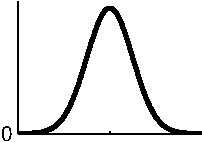
\includegraphics[width = 2cm, height = 1.5cm]{SE.pdf}}  \\

Per & $\sigma_f^2 \exp\left(-\frac{2}{\ell^2} \sin^2 \left( \pi \frac{x - x'}{p} \right)\right)$ & {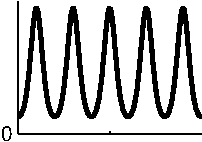
\includegraphics[width= 2 cm,height = 1.5 cm]{Per.pdf}} \\

Lin & $\sigma_f^2 (x - c)(x' - c)$ & {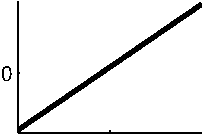
\includegraphics[width= 2 cm,height= 1.5 cm]{Lin.pdf}} \\
\hline\hline
\end{tabular}
\caption{常见的简单核函数}
\label{basickernels}
\end{table}

一般情况下将均值函数设置为零值,因为即使均值函数非零也可以在核函数$K(\mathbf{x},\mathbf{x}')$中增加一项来实现均值函数非零。

高斯过程的核(Kernel)有很多种,最常见并且最基本的核函数主要包括:平方指数(SE, Squared-Exponential)、周期(Per, Periodic)和线性(Lin, Linear)核函数,其中各核函数根据不同维度的参数是否相同分为各向同性和各向异性两种。除去以上核函数,还包括伽马指数(GE, Gamma Exponential)、有理二次(RQ, Rational Quadratic)核函数等。

然而,基本的核函数并不能表示出所有高斯过程。当需要的模型结构不能用基本核函数表达时,需要将各种基本核函数组合起来,形成新的核函数。常用的组合方法有加法、乘法和复合等。

以两个核函数$k_{a}$和$k_{b}$为例:
\[k_{a} + k_{b} = k_{a}(\mathbf{x},\mathbf{x}') + k_{b}(\mathbf{x},\mathbf{x}')\]
\[k_{a} \times k_{b} = k_{a}(\mathbf{x},\mathbf{x}') \times k_{b}(\mathbf{x},\mathbf{x}')\]
图\ref{basickernels}展示了三种基本核函数,图\ref{addkernels}展示了基本核函数之间相加组合后构成的新核函数,图\ref{mulkernels}展示了基本核函数之间相乘组合后构成的常见核函数。通过加乘方法核函数的结构表现能力得到了很大的提高。

\begin{table}[!htbp]
\centering
\begin{tabular}{c|ccc}
\hline\hline
\raisebox{0.5cm}{示意图}& {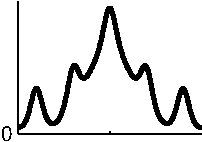
\includegraphics[width= 2 cm,height = 1.5 cm]{SE_Per_Plus.pdf}}  &  {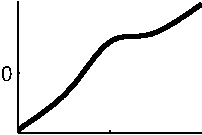
\includegraphics[width= 2 cm,height = 1.5 cm]{SE_Lin_Plus.pdf}} &  {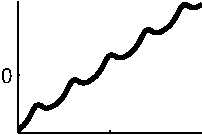
\includegraphics[width= 2 cm,height = 1.5 cm]{Lin_Per_Plus.pdf}}\\
形式 & SE+Per & SE+Lin & Lin+Per\\
\hline\hline
\end{tabular}
\caption{常见核函数相加}
\label{addkernels}
\end{table}

\begin{table}[!htbp]
\centering
\begin{tabular}{c|ccc}
\hline\hline
\raisebox{0.7cm}{示意图}& {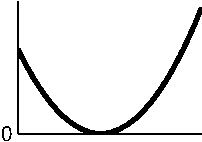
\includegraphics[width= 2.5 cm,height = 2 cm]{Lin_Lin_Mul.pdf}}  &  {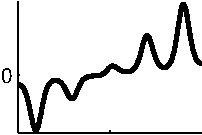
\includegraphics[width= 2.5 cm,height = 2 cm]{Lin_Per_Mul.pdf}} \\
形式 & Lin$\times$Lin & Lin$\times$Per\\ \hline
\raisebox{0.7cm}{示意图}& {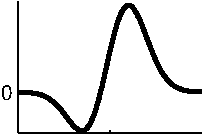
\includegraphics[width= 2.5 cm,height = 2 cm]{SE_Lin_Mul.pdf}}  &  {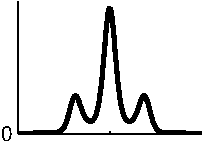
\includegraphics[width= 2.5 cm,height = 2 cm]{SE_Per_Mul.pdf}} \\
形式 & SE$\times$Lin & SE$\times$Per\\
\hline\hline
\end{tabular}
\caption{常见核函数相乘}
\label{mulkernels}
\end{table}


\subsection{边缘似然函数}

对于一组训练数据,给定某一个基本模型或者复合模型时,如何评价模型的好坏或者如何对比模型呢?在高斯过程回归中,常使用边缘似然(Marginal Likelihood)函数值评价模型与数据之间的契合程度\ref{Auto}。

在给定一组函数值$\mathbf{f}(\mathbf{x}) = [f(\mathbf{x}_{1}),f(\mathbf{x}_{2}),\cdots,f(\mathbf{x}_{N})]$的先验时,在$\mathbf{x}$处的边缘似然函数为
\[p(\mathbf{f}(\mathbf{x})\vert\mathbf{x},m(\cdot),K(\cdot,\cdot)) = N(\mathbf{f}(\mathbf{x})\vert\mathbf{x},m(\mathbf{x}),K(\mathbf{x},\mathbf{x}))\]

高斯过程回归中实际常用的似然函数(分布)有:高斯分布、Laplace分布、t分布、Gumbel分布等;对于多元高斯,常常将其密度函数作为边缘似然函数。

\section{高斯过程回归的简单应用}
本部分将实现高斯过程回归的简单应用,解决一维较少数据的模型选择问题。

\subsection{问题描述}
给定一组数据,包含xtrain、ytrain、 xtest,其中训练数据543个,测试数据87个。利用训练数据(xtrain, ytrain)训练合适的高斯过程回归模型,预测xtest上各点处的数值,并与实际观测值进行比较,计算测试数据上的MSE。

\subsection{解决思路}

本问题的核心是通过核函数的加和乘等操作,找到足以描述数据内在规律的核函数。本文为了重点体现模型建立的过程,首先使用SE、Per、Lin等基本核函数尝试对训练数据进行建模,并使用测试数据进行比较与选择;然后再运用核函数的加法乘法组合找到更能表达训练数据特征的核函数。

通过对核函数进行加、乘或函数复合等操作,可以构造非常复杂的核函数,使高斯过程回归具有强大的建模能力。在选定恰当的核函数形式后,需要通过训练数据从中估计出核函数的参数,一般可以归类为求解下面的优化问题:

\[\Theta = arg \max\ln p(y_{1},y_{2},\cdots,y_{n}\vert \mathbf{x}_{1},\mathbf{x}_{2},\cdots,\mathbf{x}_{n},\Theta)\]

\subsection{基于基本核函数的模型}
本文先尝试使用基本的核函数(Basic Kernels)对训练数据进行建模,基本核函数相对于复合形式的核函数,其表现数据内在规律的能力必然相对较弱。但是,尝试基本核函数也不是毫无用处,不仅能够大致描述出数据的结构规律,还能帮助理解高斯过程回归的一般方法,为后续基于复合核函数的模型的寻找奠定基础。

\subsubsection{方法分析}
使用基本核函数的一般步骤为\cite{frame}:

{\kaishu 
\noindent1).\quad 选定均值函数、核函数、似然函数及贝叶斯推断方式;

\noindent2).\quad 初始化均值函数、核函数的参数;

\noindent3).\quad 基于训练数据,使用求最小值的算法优化参数;

\noindent4).\quad 根据优化后的参数基于训练数据对测试数据进行预测,并使用{\rm MSE}进行评价。
}

本文此处选择均值函数为线性和常数相加的结果(一次均值函数),似然函数选择高斯似然函数,因为这样后验概率也是高斯形式(高斯分布是本身的共轭先验)。优化参数时,选择共轭梯度法求出多元函数最小值(需要注意不要陷入局部最小值)。根据以上方法和步骤,实现对训练数据的精确描述。

\subsubsection{仿真及数值结果}
本文通过仿真(Simulation)得到数值结果,对上面基于基本核函数的模型进行实现与分析对比。本文中所有仿真结果均在Windows 8.1操作系统、``intel(R) Core(TM) i5-4210U CPU @1.7GHz"下使用MATLAB R2014a进行仿真得到。

本次大作业的核心代码部分使用的是Matlab的GPML(Gaussian Process Machine Learning)函数库\footnote{\url{http://www.gaussianprocess.org/gpml/code}},不仅包括各种均值函数、核函数、似然函数,还提供了共轭梯度算法等相关函数,对本文的研究提供了很大的方便。

\begin{table}[!htbp]
\centering
\begin{tabular}{c|c|c|c|c}
\hline\hline
核函数 & SE & Lin & RQ & Per \\ \hline
MSE & 4.9326 & 51.5585 & 23.0420 & 52.1925 \\
运行时间 & 12.38s & 5.79s & 10.76s & 5.84s \\
\hline\hline
\end{tabular}
\caption{基本核函数的比较}
\label{q1basic}
\end{table}

\begin{figure}[!htbp]
    \centering
    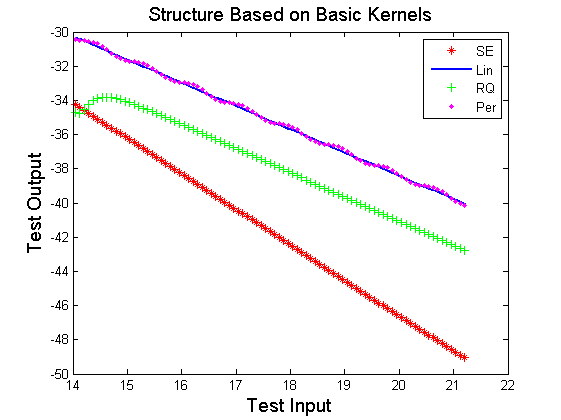
\includegraphics[width = 8 cm,height= 6.5 cm]{Q1_basic.png}
    \caption{基本核函数实现结果比较}
    \label{basiccom}
\end{figure}

\subsubsection{小结}
根据表\ref{q1basic}和图\ref{basiccom}所示的结果,可以看出:如果仅用基本的核函数而不进行核函数的复合,能够达到的最小MSE为4.9236,对应于平方指数(SE)函数。如果从运行耗费时间来看,线性(Lin)核函数和周期(Per)核函数的运行时间明显比平方指数(SE)更短。从上面结果也体现出不同核函数在表现数据结构模型时,在时间复杂度和空间复杂度上的不同特性。

上述结果同时也表明:基本核函数对数据的表示能力十分有限,为了达到更低的MSE,获得更好地回归拟合效果,多个核函数的加乘组合显得势在必行。

\subsection{基于复合核函数的模型}
对于多个核函数的复合,本次大作业最终手动选择了三种形式,分别受到\cite{GPML}第5.4节和文献\cite{Auto2}第3.6.1节Mauna Loa地区二氧化碳变化趋势的启发。将变化趋势\ref{MaunaLoa}与训练数据的示意图\ref{plottrain}对比,发现除去整体的上升/下降趋势,形状基本相同,可以选择一样的模型结构。

\begin{figure}[!htbp]
    \centering
    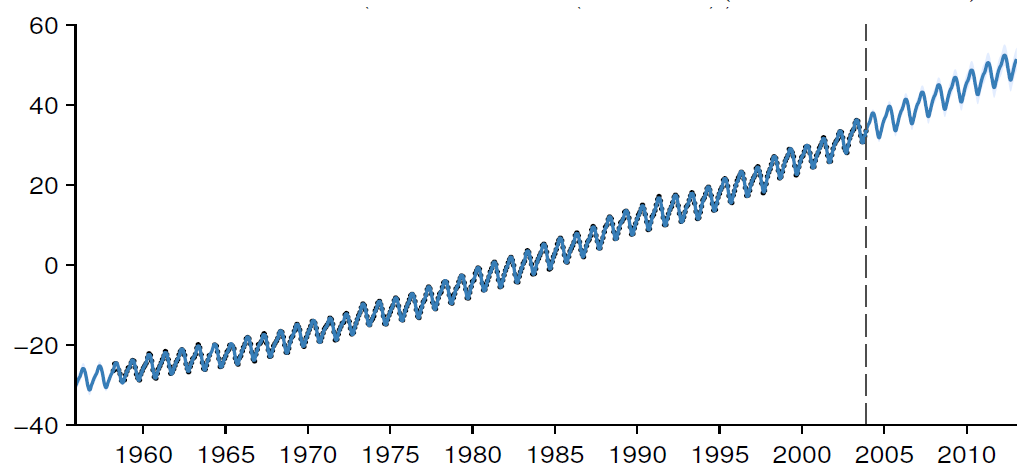
\includegraphics[width = 8 cm,height= 3.5 cm]{MaunaLoa.png}
    \caption{Mauna Loa大气$CO_{2}$浓度趋势}
    \label{MaunaLoa}
\end{figure}

\begin{figure}[!htbp]
    \centering
    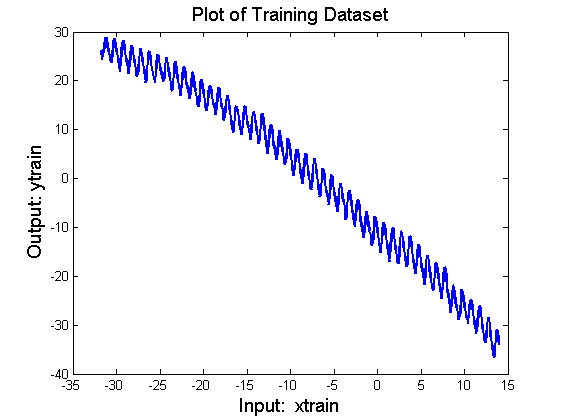
\includegraphics[width = 8 cm,height= 6.5 cm]{plot_training.png}
    \caption{训练数据输入输出关系}
    \label{plottrain}
\end{figure}


文献\cite{GPML}第5.4节中为人为选择的结果,而文献\cite{Auto2}第3.6节则使用自动选择和建立模型的方法。本文按照以上两种思路,同时尝试给出了第三种结构,并在测试数据上对建立的三个模型进行分析与比较。

\subsubsection{复合模型一}
Rusmussen和Williams在文献\cite{GPML}中对Mauna Loa地区大气二氧化碳浓度的数据变化进行了手动建模,最终结果分为四项(如表\ref{comp1}所示)。

最终构造的核函数为:
\[k(x,x') = k_{1}(x,x') + k_{2}(x,x') + k_{3}(x,x')
+ k_{4}(x,x')\]

包含的待定的超参数为$\mathbf{\theta} = (\theta_{1},\theta_{1},\cdots,\theta_{11})^{\rm T} $,然后利用GPML函数库中的共轭梯度算法(minimize函数)优化这11个参数,并使用优化后的参数对测试数据进行预测。

\begin{table}[!htbp]
\centering
\begin{tabular}{c|c|c}
\hline\hline
核 & 形式 & 具体表达式\\ \hline
$k_{1}$ & SE & $\theta_{1}^{2}\exp\left(-\frac{(x-x')^2}{2\theta_{2}^{2}}\right)$ \\ 
$k_{2}$ & SE$\times$Per & $\theta_{3}^{2}\exp\left(-\frac{(x-x')^2}{2\theta_{4}^2}-\frac{2\sin^2(\pi(x-x'))}{\theta_{5}^2}\right)$  \\
$k_{3}$ & RQ & $ \theta_{6}^2\left(1+\frac{(x-x')^2}{2\theta_{8}\theta_{7}^2}\right)^{-\theta_{8}} $  \\
$k_{4}$ & SE + WN & $ \theta_{9}^2\exp\left(-\frac{(x-x')^2}{2\theta_{10}^2}\right)+\theta_{11}^2\delta_{xx'} $  \\
\hline\hline
\end{tabular}
\caption{复合模型一}
\label{comp1}
\end{table}

\subsubsection{复合模型二}
Duvenaud在文献\cite{struct}中实现了高斯过程回归自动建立模型,自动建立的完整模型为:

\[\rm{Lin \times SE + SE \times  Per + SE \times RQ}\]

本文选择这一模型作为复合模型二,同样进行高斯过程回归的操作,并对测试数据进行预测,计算出MSE。

\subsubsection{复合模型三}
本文通过问题一训练数据的输入输出的关系图,尝试自己写出了一个由基本模型进行加法乘法运算得到的复合模型,表达式如下:

\[\rm {SE\times(LIN + RQ\times PER)}\]

\subsection{仿真与数值结果}
仿真时,根据均值函数的不同,所有模型共分为两大组,一组均值函数使用线性(Lin)与常数(Const)之和,另一组均值函数使用常数型(Const)均值函数,每组又根据核函数的不同分为前文三种复合模型。

\begin{table}[!htbp]
\centering
\begin{tabular}{c|c|c|c}
\hline\hline
复合核函数 & 模型一 & 模型二 & 模型三 \\ \hline
MSE & 6.3651 & 2.6091 & 0.2268 \\
运行时间 & 55.14s & 56.00s & 38.37s\\
\hline\hline
\end{tabular}
\caption{均值函数为Const}
\label{compmean1}
\end{table}

\begin{table}[!htbp]
\centering
\begin{tabular}{c|c|c|c}
\hline\hline
复合核函数 & 模型一 & 模型二 & 模型三 \\ \hline
MSE & 4.2619 & 1.6109 & 0.8086  \\
运行时间 & 52.44s & 53.55s & 38.38s \\
\hline\hline
\end{tabular}
\caption{均值函数为Lin+Const}
\label{compmean2}
\end{table}

{\kaishu \bf{小结:}}

对模型的评价同样有两个衡量标准:模型对测试数据预测结果的MSE
及程序运行时间。图\ref{q1composite}对比了以上不同模型对测试数据的预测结果。通过比较表\ref{compmean1}和\ref{compmean2}发现,在尝试的范围内,MSE最小和运行时间最短的模型为:均值函数为常数(Const),核函数模型为复合模型三。这是本文笔者实现的最好结果。

\begin{figure}[!htbp]
    \centering
    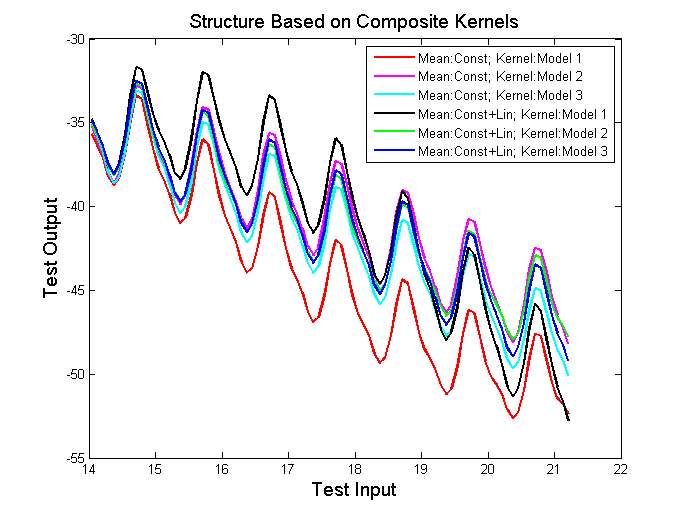
\includegraphics[width = 8 cm,height= 6.5 cm]{Q1_composite.png}
    \caption{复合模型结果比较}
    \label{q1composite}
\end{figure}

\section{高斯过程回归解决高维问题}
本次大作业第一问针对较少的一维数据进行高斯过程回归,主要困难集中在选择合适的模型。对于数据维度很高的函数,如果不能有效计算其后验分布的解析式或者计算量很大,此时获取准确的后验分布几乎不可能,因而需要采用其他的贝叶斯推断近似方法,对数据进行近似,从而减小高斯过程回归的复杂度。

\subsection{问题描述}
本次大作业第二小问提供了planecontrol.mat,数据源于F16飞机的副翼控制问题,训练数据中每一组数据包含40个分量,这些分量描述了飞机的40种状态,每组数据对应一个输出,表示该状态下采用的飞机副翼控制量。要求利用高斯过程回归,选择合适的核函数、均值函数及似然函数。并采用多种贝叶斯推断近似方法,解决飞机副翼控制问题并在测试数据上进行预测。

\subsection{解决思路}
解决了第一问之后,已经对选择核函数提供了较为清晰的思路,但是对于均值函数和似然函数的选择,尤其是贝叶斯推断的近似方法,是第二问遇到的新问题。

本文采用``尝试与比较"的思想解决这些问题,即:先给定均值和似然函数,然后尝试不同的核函数(同样包括基本核函数以及复合核函数两个方面)和贝叶斯推断近似方法,对测试数据进行预测,得到相应的MSE,最后基于MSE最小的准则对所尝试的模型进行选取。由于情况数太多,这种方法会耗费较多的时间。

\subsection{贝叶斯推断近似方法}
本文主要涉及三种贝叶斯推断近似方法,分别为Laplace近似、变分贝叶斯近似和LOO交叉验证方法。其中Laplace近似是机器学习中常用的近似算法之一,应用较为广泛。对于变分贝叶斯近似(Variational Bayesian Approximation),核心思想是使用一系列称为平滑似然函数的Laplace近似进行凸优化。

本文重点对交叉检验中的LOO(Leave-One-Out)进行分析。

\subsubsection{LOO交叉验证方法}

Leave-One-Out是一种基于交叉验证的方法,对于训练数据中$(x_{i},y_{i})$,预测的概率(取log)为:
\[\log p(y_{i}\vert \mathbf{x},\mathbf{y}_{-i},\mathbf{\theta}) = -\frac{1}{2}\log\sigma^{2}_{i} - \frac{y_{i}-\mu_{i}}{2\sigma^{2}_{i}} - \frac{1}{2}\log2\pi\]

其中$\mathbf{y}_{-i}$表示训练数据中除去第i个数据结果,$\mu$和$\sigma^2_{i}$由文献\cite{GPML}中式2.23和2.24计算。

通过以上表述,可以看出,训练数据有N个时,LOO相当于N点交叉验证,每个单独作为验证集,其余N-1个样本作为训练集,因而LOO会得到N个模型,将N个模型的最终验证集的平均数作为性能指标。

\subsection{仿真与数值结果}
在进行仿真时,由于训练数据过多,因而选择数据的一部分作为训练数据。训练数据选取多大最合适?不难得到一个明显的结论:一般情况下,训练数据越多,MSE偏向于越小,但运行时间偏向于更长,因而需要在MSE和运行时间作一个权衡。通过尝试,发现使用前1000个训练数据的效果较好。

附表中表\ref{laplace}至表\ref{LOO}使用以上三种贝叶斯推断近似方法进行高斯过程回归,并将MSE结果进行对比。表中详细给出了考虑范围内各种情况下模型的MSE及运行时间,通过比较可以发现,表\ref{Last}所示的模型具有较好的回归效果。

\begin{table}[!htbp]
\centering
\begin{tabular}{c|c|c|c}
\hline\hline
均值函数 & 似然函数 & 核函数 & 近似方法\\ \hline
常数& 高斯& SE & LOO\\
\hline\hline
\end{tabular}
\caption{选择的模型}
\label{Last}
\end{table}

\section{结论}
本文使用高斯过程回归解决了大作业的两个问题。对于第一个问题,最终选择的复合核函数为:
\[\rm {SE\times(LIN + RQ\times PER)}\]
均值函数为常数(Const),似然函数为高斯函数,最后基于测试数据得到的MSE为0.2268。
对于第二个问题(详见表\ref{Last}),最终选择的均值函数为常数(Const),核函数为SE(对应于GPML中的SEard函数),似然函数为高斯函数,贝叶斯推断方式为LOO交叉验证方法,最后基于测试数据得到的MSE为0.0266。

\section{致谢}
在猴年的最后两个星期,本人终于将本次关于高斯过程回归的大作业完成。本文代码实现部分以文献\cite{GPML}提供的GPML工具库为基础,核心的均值函数、似然函数、核函数和贝叶斯推断近似方法均由工具库提供。这一工具库对本文的研究及结论起到了很大的帮助,特向工具库的作者Carl Edward Rasmussen和Hannes Nickisch表示衷心的感谢!

\begin{thebibliography}{1}
\bibitem{GPML}
Rasmussen C E, Williams C K I. Gaussian Processes for Machine Learning (Adaptive Computation and Machine Learning)[M]. MIT Press, 2006:69-106.

\bibitem{struct}
Duvenaud D, Lloyd J R, Grosse R, et al. Structure Discovery in Nonparametric Regression through Compositional Kernel Search[J]. Creative Commons Attribution-Noncommercial-Share Alike, 2013.

\bibitem{Auto}
Lloyd J R, Duvenaud D, Grosse R, et al. Automatic construction and natural-language description of nonparametric regression models[C]. AAAI Press, 2015:1242-1250.

\bibitem{frame}
Chalupka K, Williams C K I, Murray I. A framework for evaluating approximation methods for Gaussian process regression[J]. Journal of Machine Learning Research, 2012, 14(1):333-350.

\bibitem{Auto2}
Duvenaud D. Automatic model construction with Gaussian processes[J]. 2014.

\end{thebibliography}

\onecolumn
\section{附表}
\subsection{不同近似方法结果比较}
\begin{table}[!htbp]
\centering
\begin{tabular}{c|c|c|c|c|c|c}
\hline\hline
评价标准&似然函数&均值函数&SE&Lin&SE+Lin&SE $\times$Lin\\ \hline
MSE&高斯函数&无& 0.0304 & 0.0343 & 0.0344 & 0.0284 \\
运行时间&高斯函数&无& 80.22s & 72.73s & 83.90s & 103.59s\\\hline
评价标准&似然函数&均值函数&SE&Lin&SE+Lin&SE $\times$Lin\\ \hline
MSE&高斯函数&常数&0.0270 & 0.0305 & 0.0313 & 0.1861 \\
运行时间&高斯函数&常数& 92.23s & 69.74s & 93.03s &  151.70s\\
\hline\hline
\end{tabular}
\caption{贝叶斯推断近似方法:Laplace近似}
\label{laplace}
\end{table}

\begin{table}[!htbp]
\centering
\begin{tabular}{c|c|c|c|c|c|c}
\hline\hline
评价标准&似然函数&均值函数&SE&Lin&SE+Lin&SE $\times$Lin\\ \hline
MSE&高斯函数&无&0.0326 & 0.0350 & 0.0352 & 0.9263\\
运行时间&高斯函数&无& 67.49s & 40.15s & 53.00s & 64.23s \\\hline
评价标准&似然函数&均值函数&SE&Lin&SE+Lin&SE $\times$Lin\\ \hline
MSE&高斯函数&常数& 0.0310 & 0.0310 & 0.0311 & 0.1922\\
运行时间&高斯函数&常数& 51.34s & 40.97s &  55.90s & 61.03s\\
\hline\hline
\end{tabular}
\caption{贝叶斯推断近似方法:变分贝叶斯}
\label{VB}
\end{table}

\begin{table}[!htbp]
\centering
\begin{tabular}{c|c|c|c|c|c|c}
\hline\hline
评价标准&似然函数&均值函数&SE&Lin&SE+Lin&SE $\times$Lin\\ \hline
MSE&高斯函数&无& 0.0319 & 0.0345 & 0.0351 & 0.0272 \\
运行时间&高斯函数&无& 95.71s & 71.12s & 91.53s & 110.81s \\\hline
评价标准&似然函数&均值函数&SE&Lin&SE+Lin&SE $\times$Lin\\ \hline
MSE&高斯函数&常数&  0.0266& 0.0309 & 0.0313 & 0.1545\\
运行时间&高斯函数&常数& 93.48s & 72.64s & 81.75s & 157.45s\\
\hline\hline
\end{tabular}
\caption{贝叶斯推断近似方法:LOO交叉验证}
\label{LOO}
\end{table}

\newpage
\subsection{代码清单}

\begin{table}[!htbp]
\centering
\begin{tabular}{c|c}
\hline\hline
文件 & 文件功能 \\ \hline 
GPML(文件夹) & 文献\cite{GPML}提供的MATLAB工具库 \\ \hline
Q1\_Basic.m & 问题一:基本核函数建立模型 \\
Q1\_Composite.m & 问题一:基本核函数的加、乘复合模型 \\ \hline
Q2\_Laplace.m & 问题二:Laplace近似方法 \\
Q2\_VB.m & 问题二:变分贝叶斯方法 \\
Q2\_LOO.m & 问题二: LOO交叉验证方法 \\ 
Q2\_SizeofDataset.m & 问题二:研究训练数据大小对MSE结果的影响 \\
\hline\hline
\end{tabular}
\caption{文件清单}
\label{list1}
\end{table}


\begin{table}[!htbp]
\centering
\begin{tabular}{c|c}
\hline\hline
文件 & 文件功能 \\ \hline 
question1.mat & 问题一数据 \\
MSE\_question2.p & 问题一计算MSE函数(加密pcode) \\ \hline
planecontrol.mat & F16副翼控制数据 \\
MSE\_plane\_control.p & 问题二计算MSE函数(加密pcode) \\ \hline
data\_read\_and\_MSE.m & 最优结果呈现文件 \\ 
\hline\hline
\end{tabular}
\caption{大作业提供数据文件及函数文件清单}
\label{list2}
\end{table}

\end{document}
